%-------------------------------------------------------------------------------
\section{Background and Motivation}
In this section, we first discuss the features and background of persistent memory, and the feasibility to replace DRAM with persistent memory. We also present the background and the design of RocksDB~\cite{RocksDB}, providing the limitations of RocksDB.
%-------------------------------------------------------------------------------
\subsection{Persistent Memory}
Persistent Memory, also known as Non-volatile memory(NVM), is a byte-addressable persistent storage device between DRAM and disk in the heterogeneous memory hierarchy. PM can be attached to a memory bus socket just like DRAM, which enables it to be accessed via load and store instructions. Modern PM technologies include phase change memory (PCM)~\cite{PCM}, memristors and 3D XPoint~\cite{3DXPoint}.

Embracing the feature of byte-addressability, PM achieves a comparable read performance with DRAM. However, the write latency of PM is about 10x higher than DRAM~\cite{DBLP:conf/usenix/XiaJXS17}, but the cost of PM is lower than DRAM. These properties make PM a suitable choice for replacing DRAM.

Since the PM can be connected via a memory bus with byte-addressable feature, the PM supports atomic writes of 8 bytes~\cite{DBLP:conf/fast/LeeLSNN17}. Compared with the traditional storage devices using block access, PM supports more fine-grained writes. When writing persistent data, we need to ensure that the data structure is consistent, even in the event of system crash. However, modern CPUs have multiple caches and in some cases, CPUs may reorder some of the memory write instructions to improve write performance, which may lead to inconsistent system state. To keep the PM write order and data structure consistent, we need to explicitly use instructions such as \textbf{MFENCE} and \textbf{CLFLUSH} (Intel x86)~\cite{SLMDB,DBLP:conf/fast/LeeLSNN17,DBLP:conf/usenix/KannanBGAA18} to make memory writes ordered and consistent. In addition, in the case where the size of the data written to the PM is greater than 8 bytes, if the system crashs and performs recovery, the recovered data structure may be partially updated, resulting in inconsistent state. Techniques such as logging and Copy-on-Write (CoW) can be used to handle this situation.


As a new storage device, PM offers new opportunities and research directions for optimizing KV stores. There are previous studies~\cite{NVMRocks,DBLP:conf/usenix/KannanBGAA18,DBLP:conf/usenix/XiaJXS17} that use PM in KV stores to optimize system performance, which requires to redesign the data structure, such as skiplist~\cite{DBLP:conf/usenix/KannanBGAA18, SLMDB}. In this work, in addition to redesigning RocksDB's~\cite{RocksDB} skiplist, we also introduce DRAM-based cache, which works with PM collaboratively to optimize the performance of the system.
\subsection{RocksDB}
\textbf{RocksDB}~\cite{RocksDB} is a persistent Key-Value store based on Log Structured Merge Tree (LSM-tree)~\cite{LSM-tree}. The architecture is shown in Figure \ref{fig:rocksdb}. LSM-tree consists of two parts: memory and Disk. In memory component, in order to improve the write throughput and change the random write to disk into sequential write, RocksDB first constructs a memory table (memtable) buffer in memory to batch write. The memtable is composed of sorted skiplist. When the data of the memtable reaches a threshold, the memtable is set to immutable, and then a new memtable is created to receive the write request. The immutable table will be flushed to disk through background thread. The disk component consists of multi-level sorted string tables (SSTable), from lowest $L_0$ to highest $L_n$. Except $L_0$, each level has one or more sorted SSTable files, where the key ranges of files at the same level do not overlap. The capacity of each level is limited, but the higher level can contain more SSTable files. The capacity of such a level is generally about 10 times larger than that of the previous level. In order to maintain such hierarchical level and data order, when the size of a level exceeds its limitation, the background thread will perform a merge sort operation (compaction) on the level and the next level, and the data of the two levels will be sorted according to the key value. When the two levels have the same key, the value of the lower level will cover the value of the higher level, so as to ensure the uniqueness of each level's data. (except $L_0$, because immutable memtable is not compacted when it is flushed to disk to increase write throughput, SSTables in $L_0$ can have overlapping key ranges.) Generally speaking, LSM-tree optimizes the write operation and sacrifices certain read performance. However, due to the multi-level structure and data order, the read operation still maintains good performance.
\begin{figure}
    \centering
    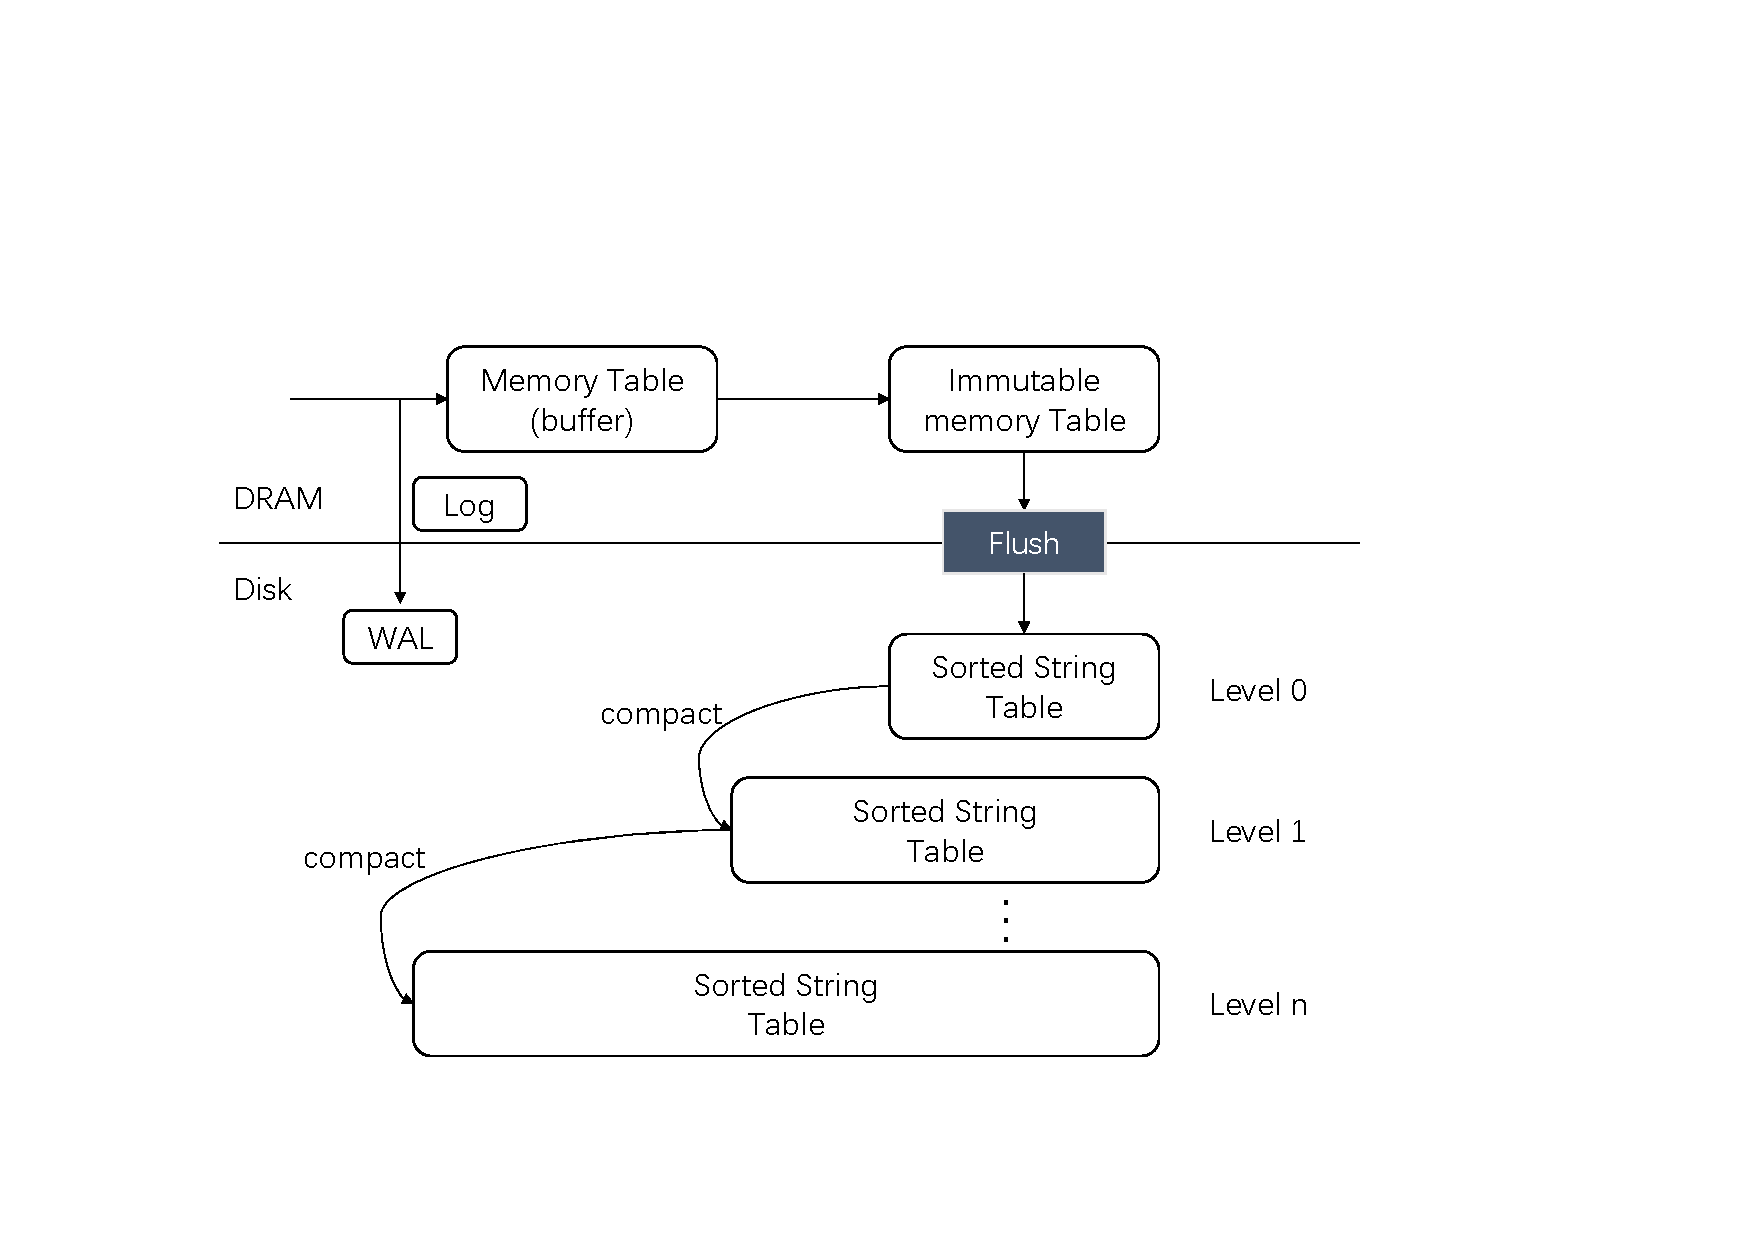
\includegraphics[width=0.36\paperwidth]{figure/rocksdb.pdf}
    \caption{RocksDB architecture.}
    \label{fig:rocksdb}
\end{figure}


\textbf{Write-Ahead-Log overhead} In order to ensure that the system can recover from crash, the write operation will be written to Write-Ahead-Log (WAL) before writing memtable. The log will be deleted after the immutable memtable is finally flushed to the disk. This can cause write performance degradation. When using \texttt{fsync()} for WAL and inserting 8GB of data with 1KB value size to create database, the write performance is reduced by more than 12 times~\cite{SLMDB}. Therefore, the trade-off of performance and consistency is involved here. By default, RocksDB does not log operations to get better performance, so some data may be lost when crash occurs. 

\textbf{Read amplification in transaction} For transactional support, RocksDB supports both Two-Phase Locking (2PL) and Optimistic Concurrency Control (OCC). For 2PL, RocksDB uses a in-memory dedicated locking manager to maintain the locks, decoupling the records with locks. When accessing a record, the manager should be accessed first to acquire lock. 

Because of multi-level structure in LSM-tree, RocksDB has the problem of read amplification~\cite{WiscKey,NVMKV,PebblesDB}. When read operation occurs, it first accesses the memtable, then the immutable memtable. If the data is not in memory, it needs to access the SSTable on disk from the lowest level to the highest level. In each level, it first uses the binary search to find the SSTable where the data is located, after identifying the SSTable, it use another binary search to find the index of the data. Therefore, when retrieving a certain level, at least two binary searches are needed. If the current level cannot retrieve the data, it will go to the next level to search, and repeat the above operations until the data is found, so the overhead of read operation on disk is high. In order to reduce the overhead of accessing the disk, RocksDB uses the Bloom filter to optimize the read operation.

For OCC, verification of records on disk is slow due to the multiple levels on the disk. RocksDB uses the minimum sequence number in memory and global sequence to determine whether to validate in memory. If the sequence is not in memory, the transaction will abort to avoid disk access. In order to optimize the read amplification problem and reduce the probability of transaction abort, we use DRAM-based cache to maintain the sequence number of outstanding transactions, so that we can validate the sequence number in DRAM-based cache when the version cannot be retrieved in memory during the validation phase, instead of accessing the disk.
